\section{Using CIG Code from Git}

\begin{frame}[plain,noframenumbering]
 \vfill
 \begin{center}
  \LARGE \color{solarizedAccent} Using CIG Code from Git
 \end{center}
 \vfill
\end{frame}

\begin{frame}
 \frametitle{Using CIG Code from Git(Hub)}

 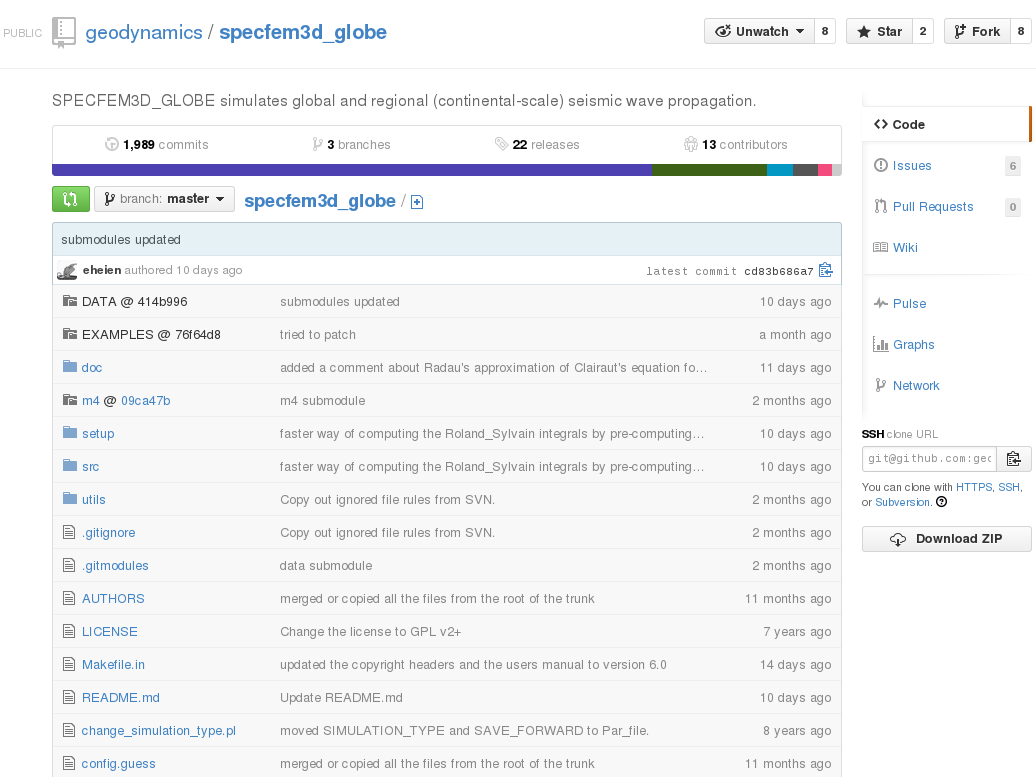
\includegraphics[height=\textheight,width=\textwidth,keepaspectratio]{github}
\end{frame}

\begin{frame}[fragile]
 \frametitle{Using CIG Code from Git}

 \begin{exampleblock}{Cloning Stable Code}
  \begin{semiverbatim}
\command{git clone \alert<2>{-{}-recursive} \\
   https://github.com/geodynamics/specfem3d_globe.git}
Cloning into `specfem3d_globe'...
remote: Reusing existing pack: 20478, done.
remote: Counting objects: 59, done.
remote: Compressing objects: 100% (59/59), done.
done.
Checking out files: 100% (701/701), done.
...
\end{semiverbatim}
 \end{exampleblock}
\end{frame}

\begin{frame}[fragile]
 \frametitle{Using CIG Code from Git}

 \begin{exampleblock}{Cloning Development Code}
  \begin{semiverbatim}
\command{git clone -{}-recursive \alert{-{}-branch devel} \\
   https://github.com/geodynamics/specfem3d_globe.git}
Cloning into `specfem3d_globe'...
remote: Reusing existing pack: 20478, done.
remote: Counting objects: 59, done.
remote: Compressing objects: 100% (59/59), done.
done.
Checking out files: 100% (701/701), done.
...
\end{semiverbatim}
 \end{exampleblock}
\end{frame}

\begin{frame}[fragile]
 \frametitle{Using CIG Code from Git}

 \begin{exampleblock}<only@1>{Switching Branches}
  \begin{semiverbatim}
\comment{Create branch that tracks upstream}
\command{git branch -{}-track devel origin/devel}
Branch origin/devel set up to track local branch \makebox[0.85\width][l]{devel}

\comment{Switch to branch}
\command{git checkout devel}
Switched to branch `devel'
Your branch is up-to-date with `origin/devel'.
\end{semiverbatim}
 \end{exampleblock}

 \begin{exampleblock}<only@2->{Shortcut}
  \begin{semiverbatim}
\comment{Create and switch to branch devel}
\command{git checkout \alert<3>{-{}-track} \alert<2>{-b devel} origin/devel}
Branch origin/devel set up to track local branch \makebox[0.85\width][l]{devel}
Switched to branch `devel'
\end{semiverbatim}
 \end{exampleblock}
\end{frame}

\begin{frame}[fragile]
 \frametitle{Using CIG Code from Git}

 \begin{exampleblock}{Fetching Updates}
  \begin{semiverbatim}
\command{git fetch \only<2>{origin}}
remote: Counting objects: 85, done.
remote: Compressing objects: 100% (85/85), done.
remote: Total 85 (delta 37), reused 2 (delta 0)
Unpacking objects: 100% (85/85), done.
From https://github.com/geodynamics/specfem3d_globe
   c45b60b..f218984  devel      -> origin/devel
\end{semiverbatim}
 \end{exampleblock}
\end{frame}

\begin{frame}[fragile,t]
 \frametitle{Using CIG Code from Git}

 \begin{exampleblock}{Reviewing Updates}
  \begin{semiverbatim}
\comment{Log starting at HEAD}
\command{git log}
\hiYellow{commit 28789049bdcb5d51cbef122842a5e1bf9cd7376d}
Merge: fedf291 2f0c52e
Author: Dimitri Komatitsch <komatits@...>
Date:   Thu May 1 09:48:38 2014 +0200

    Merge pull request \#62 from QuLogic/typos

    Fix some small typos.
\end{semiverbatim}
 \end{exampleblock}
\end{frame}

\begin{frame}[fragile,t]
 \frametitle{Using CIG Code from Git}

 \begin{exampleblock}{Reviewing Updates}
  \vspace{-1em}
  \begin{semiverbatim}
\comment{Log of changes with differences}
\command{git log -{}-patch} \comment{or -p}
\hiYellow{commit 2f0c52e3555c6d534baf40084c5f59f7fd6bc7bc}
Author: Elliott Sales de Andrade <...>
Date:   Wed Apr 30 23:32:33 2014 -0400
    Fix some small typos.
diff --git a/src/auxiliaries/combine_paraview_strain_
index 4c1fe2a..ea6d238 100644
--- a/src/auxiliaries/combine_paraview_strain_data.f9
+++ b/src/auxiliaries/combine_paraview_strain_data.f9
@@ -106,3 +106,3 @@ program combine_paraview_movie_da
\hiRed{-  ! open paraview output mesh file}
\hiGreen{+  ! open Paraview output mesh file}
     write(mesh_file,'(a,a,a,i6.6,a)')  'movie3D_',tr
\end{semiverbatim}
 \end{exampleblock}
\end{frame}

\begin{frame}[fragile,t]
 \frametitle{Using CIG Code from Git}

 \begin{exampleblock}{Reviewing Updates}
  \vspace{-1em}
  \begin{semiverbatim}
\comment{Log of changes with statistics}
\command{git log -{}-stat}
\hiYellow{commit 2f0c52e3555c6d534baf40084c5f59f7fd6bc7bc}
Author: Elliott Sales de Andrade <...>
Date:   Wed Apr 30 23:32:33 2014 -0400
    Fix some small typos.

 src/auxiliaries/combine_surf_data.f90      | 4 \hiGreen{+}\hiRed{-}
 src/auxiliaries/combine_vol_data.F90       |18 \hiGreen{++}\hiRed{-{}-}
 src/auxiliaries/create_movie_AVS_DX.f90    | 6 \hiGreen{+}\hiRed{-}
 src/auxiliaries/create_movie_GMT_global.f90|10 \hiGreen{+}\hiRed{-{}-}
 src/cuda/assemble_MPI_scalar_cuda.cu       |10 \hiGreen{+}\hiRed{-{}-}
 src/cuda/assemble_MPI_vector_cuda.cu       |14 \hiGreen{+}\hiRed{-{}-}
 src/cuda/check_fields_cuda.cu              | 2 \hiGreen{+}\hiRed{-}
\end{semiverbatim}
 \end{exampleblock}
\end{frame}

\begin{frame}[fragile,t]
 \frametitle{Using CIG Code from Git}

 \begin{exampleblock}{Reviewing Updates}
  \begin{semiverbatim}
\comment{Log starting at HEAD -- Short}
\command{git log -{}-oneline}
\hiYellow{2878904} Merge pull request \#62 from QuLogic/typos
\hiYellow{2f0c52e} Fix some small typos.
\hiYellow{fedf291} Merge pull request \#61 from QuLogic/regular-k
\hiYellow{6cea702} Save some memory on addressing array.
\hiYellow{433edf7} Use addressing to find regular grid slices.
\hiYellow{eeeeb36} Round chunk_map output to the nearest EPS.
\hiYellow{672b5e6} Use specfem modules to reduce subroutine argu
\hiYellow{811ae11} Merge pull request \#60 from komatits/devel
\hiYellow{163240c} simpler implementation of volume and area cal
\hiYellow{32686e3} Fix allocation of regular kernel arrays.
\hiYellow{e27d871} Merge pull request \#59 from komatits/devel
\end{semiverbatim}
 \end{exampleblock}
\end{frame}

\begin{frame}[fragile,t]
 \frametitle{Using CIG Code from Git}

 \begin{exampleblock}{Reviewing Updates}
  \begin{semiverbatim}
\comment{Log of new changes}
\command{git log -{}-oneline devel..origin/devel}
\hiYellow{f218984} Merge pull request #88 from komatits/devel
\hiYellow{a5dde6d} added an email from Daniel Peter about ellipt
\hiYellow{f2de2cd} Merge pull request #87 from komatits/devel
\hiYellow{ffd536a} renamed model_crust to model_crust_2_0 to be
\hiYellow{e63245c} Merge pull request #86 from komatits/devel
\hiYellow{2614dd9} done cleaning and adding all the topography
\hiYellow{ba3f67c} Merge pull request #85 from komatits/devel
\hiYellow{04ab1bc} replaced the old version of ETOPO with the
\hiYellow{97da690} Merge pull request #84 from komatits/devel
\hiYellow{85124e8} compressed the large topo files that are
\hiYellow{0e84408} Merge pull request #83 from komatits/devel
\end{semiverbatim}
 \end{exampleblock}
\end{frame}

\begin{frame}[fragile]
 \frametitle{Using CIG Code from Git}

 \begin{exampleblock}{Merge Updates}
  \begin{semiverbatim}
\command{git merge \only<2>{origin/master}}
Updating c45b60b..f218984
Fast-forward
...
\end{semiverbatim}
 \end{exampleblock}
\end{frame}
